\documentclass[1p]{elsarticle_modified}
%\bibliographystyle{elsarticle-num}

%\usepackage[colorlinks]{hyperref}
%\usepackage{abbrmath_seonhwa} %\Abb, \Ascr, \Acal ,\Abf, \Afrak
\usepackage{amsfonts}
\usepackage{amssymb}
\usepackage{amsmath}
\usepackage{amsthm}
\usepackage{scalefnt}
\usepackage{amsbsy}
\usepackage{kotex}
\usepackage{caption}
\usepackage{subfig}
\usepackage{color}
\usepackage{graphicx}
\usepackage{xcolor} %% white, black, red, green, blue, cyan, magenta, yellow
\usepackage{float}
\usepackage{setspace}
\usepackage{hyperref}

\usepackage{tikz}
\usetikzlibrary{arrows}

\usepackage{multirow}
\usepackage{array} % fixed length table
\usepackage{hhline}

%%%%%%%%%%%%%%%%%%%%%
\makeatletter
\renewcommand*\env@matrix[1][\arraystretch]{%
	\edef\arraystretch{#1}%
	\hskip -\arraycolsep
	\let\@ifnextchar\new@ifnextchar
	\array{*\c@MaxMatrixCols c}}
\makeatother %https://tex.stackexchange.com/questions/14071/how-can-i-increase-the-line-spacing-in-a-matrix
%%%%%%%%%%%%%%%

\usepackage[normalem]{ulem}

\newcommand{\msout}[1]{\ifmmode\text{\sout{\ensuremath{#1}}}\else\sout{#1}\fi}
%SOURCE: \msout is \stkout macro in https://tex.stackexchange.com/questions/20609/strikeout-in-math-mode

\newcommand{\cancel}[1]{
	\ifmmode
	{\color{red}\msout{#1}}
	\else
	{\color{red}\sout{#1}}
	\fi
}

\newcommand{\add}[1]{
	{\color{blue}\uwave{#1}}
}

\newcommand{\replace}[2]{
	\ifmmode
	{\color{red}\msout{#1}}{\color{blue}\uwave{#2}}
	\else
	{\color{red}\sout{#1}}{\color{blue}\uwave{#2}}
	\fi
}

\newcommand{\Sol}{\mathcal{S}} %segment
\newcommand{\D}{D} %diagram
\newcommand{\A}{\mathcal{A}} %arc


%%%%%%%%%%%%%%%%%%%%%%%%%%%%%5 test

\def\sl{\operatorname{\textup{SL}}(2,\Cbb)}
\def\psl{\operatorname{\textup{PSL}}(2,\Cbb)}
\def\quan{\mkern 1mu \triangleright \mkern 1mu}

\theoremstyle{definition}
\newtheorem{thm}{Theorem}[section]
\newtheorem{prop}[thm]{Proposition}
\newtheorem{lem}[thm]{Lemma}
\newtheorem{ques}[thm]{Question}
\newtheorem{cor}[thm]{Corollary}
\newtheorem{defn}[thm]{Definition}
\newtheorem{exam}[thm]{Example}
\newtheorem{rmk}[thm]{Remark}
\newtheorem{alg}[thm]{Algorithm}

\newcommand{\I}{\sqrt{-1}}
\begin{document}

%\begin{frontmatter}
%
%\title{Boundary parabolic representations of knots up to 8 crossings}
%
%%% Group authors per affiliation:
%\author{Yunhi Cho} 
%\address{Department of Mathematics, University of Seoul, Seoul, Korea}
%\ead{yhcho@uos.ac.kr}
%
%
%\author{Seonhwa Kim} %\fnref{s_kim}}
%\address{Center for Geometry and Physics, Institute for Basic Science, Pohang, 37673, Korea}
%\ead{ryeona17@ibs.re.kr}
%
%\author{Hyuk Kim}
%\address{Department of Mathematical Sciences, Seoul National University, Seoul 08826, Korea}
%\ead{hyukkim@snu.ac.kr}
%
%\author{Seokbeom Yoon}
%\address{Department of Mathematical Sciences, Seoul National University, Seoul, 08826,  Korea}
%\ead{sbyoon15@snu.ac.kr}
%
%\begin{abstract}
%We find all boundary parabolic representation of knots up to 8 crossings.
%
%\end{abstract}
%\begin{keyword}
%    \MSC[2010] 57M25 
%\end{keyword}
%
%\end{frontmatter}

%\linenumbers
%\tableofcontents
%
\newcommand\colored[1]{\textcolor{white}{\rule[-0.35ex]{0.8em}{1.4ex}}\kern-0.8em\color{red} #1}%
%\newcommand\colored[1]{\textcolor{white}{ #1}\kern-2.17ex	\textcolor{white}{ #1}\kern-1.81ex	\textcolor{white}{ #1}\kern-2.15ex\color{red}#1	}

{\Large $\underline{12a_{1242}~(K12a_{1242})}$}

\setlength{\tabcolsep}{10pt}
\renewcommand{\arraystretch}{1.6}
\vspace{1cm}\begin{tabular}{m{100pt}>{\centering\arraybackslash}m{274pt}}
\multirow{5}{120pt}{
	\centering
	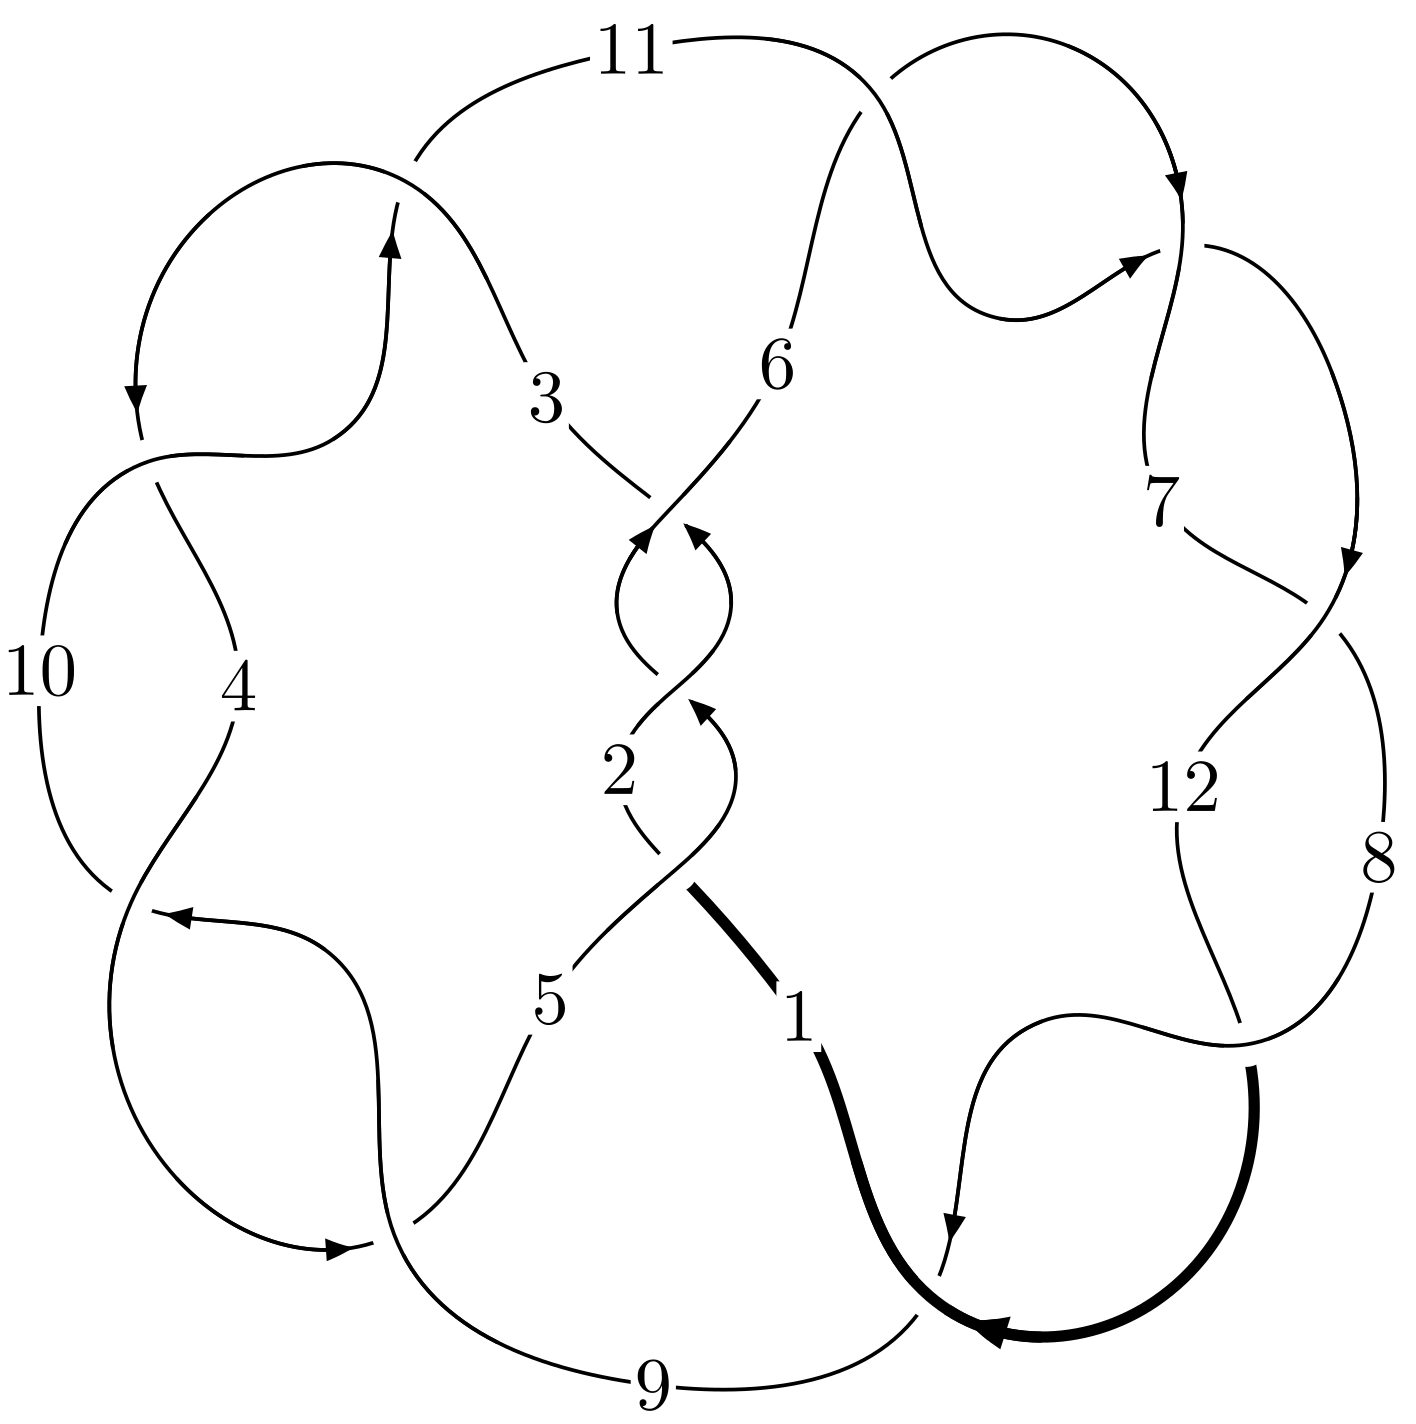
\includegraphics[width=112pt]{../../../GIT/diagram.site/Diagrams/png/2043_12a_1242.png}\\
\ \ \ A knot diagram\footnotemark}&
\allowdisplaybreaks
\textbf{Linearized knot diagam} \\
\cline{2-2}
 &
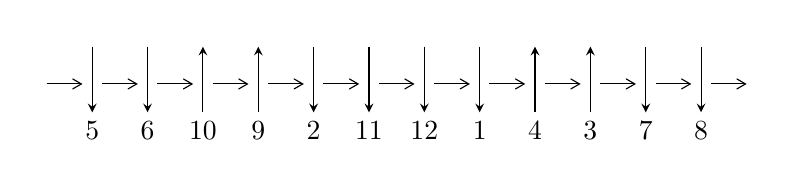
\begin{tikzpicture}[x=20pt, y=17pt]
	% nodes
	\node (C0) at (0, 0) {};
	\node (C1) at (1, 0) {};
	\node (C1U) at (1, +1) {};
	\node (C1D) at (1, -1) {5};

	\node (C2) at (2, 0) {};
	\node (C2U) at (2, +1) {};
	\node (C2D) at (2, -1) {6};

	\node (C3) at (3, 0) {};
	\node (C3U) at (3, +1) {};
	\node (C3D) at (3, -1) {10};

	\node (C4) at (4, 0) {};
	\node (C4U) at (4, +1) {};
	\node (C4D) at (4, -1) {9};

	\node (C5) at (5, 0) {};
	\node (C5U) at (5, +1) {};
	\node (C5D) at (5, -1) {2};

	\node (C6) at (6, 0) {};
	\node (C6U) at (6, +1) {};
	\node (C6D) at (6, -1) {11};

	\node (C7) at (7, 0) {};
	\node (C7U) at (7, +1) {};
	\node (C7D) at (7, -1) {12};

	\node (C8) at (8, 0) {};
	\node (C8U) at (8, +1) {};
	\node (C8D) at (8, -1) {1};

	\node (C9) at (9, 0) {};
	\node (C9U) at (9, +1) {};
	\node (C9D) at (9, -1) {4};

	\node (C10) at (10, 0) {};
	\node (C10U) at (10, +1) {};
	\node (C10D) at (10, -1) {3};

	\node (C11) at (11, 0) {};
	\node (C11U) at (11, +1) {};
	\node (C11D) at (11, -1) {7};

	\node (C12) at (12, 0) {};
	\node (C12U) at (12, +1) {};
	\node (C12D) at (12, -1) {8};
	\node (C13) at (13, 0) {};

	% arrows
	\draw[->,>={angle 60}]
	(C0) edge (C1) (C1) edge (C2) (C2) edge (C3) (C3) edge (C4) (C4) edge (C5) (C5) edge (C6) (C6) edge (C7) (C7) edge (C8) (C8) edge (C9) (C9) edge (C10) (C10) edge (C11) (C11) edge (C12) (C12) edge (C13) ;	\draw[->,>=stealth]
	(C1U) edge (C1D) (C2U) edge (C2D) (C3D) edge (C3U) (C4D) edge (C4U) (C5U) edge (C5D) (C6U) edge (C6D) (C7U) edge (C7D) (C8U) edge (C8D) (C9D) edge (C9U) (C10D) edge (C10U) (C11U) edge (C11D) (C12U) edge (C12D) ;
	\end{tikzpicture} \\
\hhline{~~} \\& 
\textbf{Solving Sequence} \\ \cline{2-2} 
 &
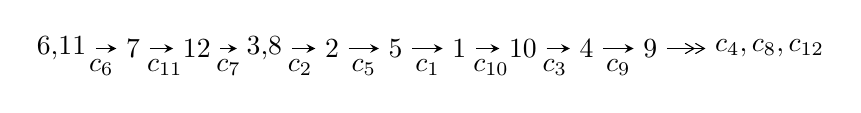
\begin{tikzpicture}[x=23pt, y=7pt]
	% node
	\node (A0) at (-1/8, 0) {6,11};
	\node (A1) at (1, 0) {7};
	\node (A2) at (2, 0) {12};
	\node (A3) at (49/16, 0) {3,8};
	\node (A4) at (33/8, 0) {2};
	\node (A5) at (41/8, 0) {5};
	\node (A6) at (49/8, 0) {1};
	\node (A7) at (57/8, 0) {10};
	\node (A8) at (65/8, 0) {4};
	\node (A9) at (73/8, 0) {9};
	\node (C1) at (1/2, -1) {$c_{6}$};
	\node (C2) at (3/2, -1) {$c_{11}$};
	\node (C3) at (5/2, -1) {$c_{7}$};
	\node (C4) at (29/8, -1) {$c_{2}$};
	\node (C5) at (37/8, -1) {$c_{5}$};
	\node (C6) at (45/8, -1) {$c_{1}$};
	\node (C7) at (53/8, -1) {$c_{10}$};
	\node (C8) at (61/8, -1) {$c_{3}$};
	\node (C9) at (69/8, -1) {$c_{9}$};
	\node (A10) at (11, 0) {$c_{4},c_{8},c_{12}$};

	% edge
	\draw[->,>=stealth]	
	(A0) edge (A1) (A1) edge (A2) (A2) edge (A3) (A3) edge (A4) (A4) edge (A5) (A5) edge (A6) (A6) edge (A7) (A7) edge (A8) (A8) edge (A9) ;
	\draw[->>,>={angle 60}]	
	(A9) edge (A10);
\end{tikzpicture} \\ 

\end{tabular} \\

\footnotetext{
The image of knot diagram is generated by the software ``\textbf{Draw programme}" developed by Andrew Bartholomew(\url{http://www.layer8.co.uk/maths/draw/index.htm\#Running-draw}), where we modified some parts for our purpose(\url{https://github.com/CATsTAILs/LinksPainter}).
}\phantom \\ \newline 
\centering \textbf{Ideals for irreducible components\footnotemark of $X_{\text{par}}$} 
 
\begin{align*}
I^u_{1}&=\langle 
-73684140 u^{28}-84869082 u^{27}+\cdots+145070621 b-231458335,\\
\phantom{I^u_{1}}&\phantom{= \langle  }109671719 u^{28}+211321507 u^{27}+\cdots+870423726 a+469996164,\;u^{29}+2 u^{28}+\cdots+3 u+3\rangle \\
I^u_{2}&=\langle 
b-1,\;a^2-2 u+4,\;u^2- u-1\rangle \\
I^u_{3}&=\langle 
b+1,\;a,\;u^2+u-1\rangle \\
\\
\end{align*}
\raggedright * 3 irreducible components of $\dim_{\mathbb{C}}=0$, with total 35 representations.\\
\footnotetext{All coefficients of polynomials are rational numbers. But the coefficients are sometimes approximated in decimal forms when there is not enough margin.}
\newpage
\renewcommand{\arraystretch}{1}
\centering \section*{I. $I^u_{1}= \langle -7.37\times10^{7} u^{28}-8.49\times10^{7} u^{27}+\cdots+1.45\times10^{8} b-2.31\times10^{8},\;1.10\times10^{8} u^{28}+2.11\times10^{8} u^{27}+\cdots+8.70\times10^{8} a+4.70\times10^{8},\;u^{29}+2 u^{28}+\cdots+3 u+3 \rangle$}
\flushleft \textbf{(i) Arc colorings}\\
\begin{tabular}{m{7pt} m{180pt} m{7pt} m{180pt} }
\flushright $a_{6}=$&$\begin{pmatrix}1\\0\end{pmatrix}$ \\
\flushright $a_{11}=$&$\begin{pmatrix}0\\u\end{pmatrix}$ \\
\flushright $a_{7}=$&$\begin{pmatrix}1\\u^2\end{pmatrix}$ \\
\flushright $a_{12}=$&$\begin{pmatrix}- u\\- u^3+u\end{pmatrix}$ \\
\flushright $a_{3}=$&$\begin{pmatrix}-0.125998 u^{28}-0.242780 u^{27}+\cdots-2.67848 u-0.539962\\0.507919 u^{28}+0.585019 u^{27}+\cdots-1.09278 u+1.59549\end{pmatrix}$ \\
\flushright $a_{8}=$&$\begin{pmatrix}- u^2+1\\- u^4+2 u^2\end{pmatrix}$ \\
\flushright $a_{2}=$&$\begin{pmatrix}0.381921 u^{28}+0.342239 u^{27}+\cdots-3.77126 u+1.05552\\0.507919 u^{28}+0.585019 u^{27}+\cdots-1.09278 u+1.59549\end{pmatrix}$ \\
\flushright $a_{5}=$&$\begin{pmatrix}-0.468112 u^{28}-0.582646 u^{27}+\cdots+3.90750 u-1.40739\\-0.374870 u^{28}-0.400564 u^{27}+\cdots+1.59469 u-1.19585\end{pmatrix}$ \\
\flushright $a_{1}=$&$\begin{pmatrix}u^3-2 u\\u^5-3 u^3+u\end{pmatrix}$ \\
\flushright $a_{10}=$&$\begin{pmatrix}0.277134 u^{28}+0.150852 u^{27}+\cdots+1.79663 u+1.03838\\0.00440318 u^{28}+0.00821410 u^{27}+\cdots+0.0681851 u+0.279727\end{pmatrix}$ \\
\flushright $a_{4}=$&$\begin{pmatrix}0.346692 u^{28}+0.461594 u^{27}+\cdots-4.19855 u+1.50586\\0.258251 u^{28}+0.340383 u^{27}+\cdots-1.54868 u+1.00040\end{pmatrix}$ \\
\flushright $a_{9}=$&$\begin{pmatrix}u^4-3 u^2+1\\u^6-4 u^4+3 u^2\end{pmatrix}$\\&\end{tabular}
\flushleft \textbf{(ii) Obstruction class $= -1$}\\~\\
\flushleft \textbf{(iii) Cusp Shapes $= \frac{293684115}{145070621} u^{28}+\frac{473769543}{145070621} u^{27}+\cdots-\frac{27583342}{145070621} u+\frac{376643745}{145070621}$}\\~\\
\newpage\renewcommand{\arraystretch}{1}
\flushleft \textbf{(iv) u-Polynomials at the component}\newline \\
\begin{tabular}{m{50pt}|m{274pt}}
Crossings & \hspace{64pt}u-Polynomials at each crossing \\
\hline $$\begin{aligned}c_{1},c_{2},c_{5}\end{aligned}$$&$\begin{aligned}
&u^{29}+3 u^{28}+\cdots-4 u+11
\end{aligned}$\\
\hline $$\begin{aligned}c_{3},c_{4},c_{9}\\c_{10}\end{aligned}$$&$\begin{aligned}
&u^{29}+u^{28}+\cdots+8 u+4
\end{aligned}$\\
\hline $$\begin{aligned}c_{6},c_{7},c_{8}\\c_{11},c_{12}\end{aligned}$$&$\begin{aligned}
&u^{29}-2 u^{28}+\cdots+3 u-3
\end{aligned}$\\
\hline
\end{tabular}\\~\\
\newpage\renewcommand{\arraystretch}{1}
\flushleft \textbf{(v) Riley Polynomials at the component}\newline \\
\begin{tabular}{m{50pt}|m{274pt}}
Crossings & \hspace{64pt}Riley Polynomials at each crossing \\
\hline $$\begin{aligned}c_{1},c_{2},c_{5}\end{aligned}$$&$\begin{aligned}
&y^{29}-35 y^{28}+\cdots+2018 y-121
\end{aligned}$\\
\hline $$\begin{aligned}c_{3},c_{4},c_{9}\\c_{10}\end{aligned}$$&$\begin{aligned}
&y^{29}+39 y^{28}+\cdots+96 y-16
\end{aligned}$\\
\hline $$\begin{aligned}c_{6},c_{7},c_{8}\\c_{11},c_{12}\end{aligned}$$&$\begin{aligned}
&y^{29}-42 y^{28}+\cdots+93 y-9
\end{aligned}$\\
\hline
\end{tabular}\\~\\
\newpage\flushleft \textbf{(vi) Complex Volumes and Cusp Shapes}
$$\begin{array}{c|c|c}  
\text{Solutions to }I^u_{1}& \I (\text{vol} + \sqrt{-1}CS) & \text{Cusp shape}\\
 \hline 
\begin{aligned}
u &= -0.957238 + 0.092408 I \\
a &= \phantom{-}0.133281 + 0.801704 I \\
b &= \phantom{-}0.518624 - 0.562490 I\end{aligned}
 & -3.64717 + 1.99860 I & -12.92483 - 5.25598 I \\ \hline\begin{aligned}
u &= -0.957238 - 0.092408 I \\
a &= \phantom{-}0.133281 - 0.801704 I \\
b &= \phantom{-}0.518624 + 0.562490 I\end{aligned}
 & -3.64717 - 1.99860 I & -12.92483 + 5.25598 I \\ \hline\begin{aligned}
u &= -0.417915 + 0.773611 I \\
a &= -1.69685 + 0.96816 I \\
b &= \phantom{-}1.64439 - 0.07500 I\end{aligned}
 & -14.7963 + 2.4842 I & -12.51838 - 2.49231 I \\ \hline\begin{aligned}
u &= -0.417915 - 0.773611 I \\
a &= -1.69685 - 0.96816 I \\
b &= \phantom{-}1.64439 + 0.07500 I\end{aligned}
 & -14.7963 - 2.4842 I & -12.51838 + 2.49231 I \\ \hline\begin{aligned}
u &= \phantom{-}1.18567\phantom{ +0.000000I} \\
a &= \phantom{-}0.637942\phantom{ +0.000000I} \\
b &= \phantom{-}1.42557\phantom{ +0.000000I}\end{aligned}
 & -7.33093\phantom{ +0.000000I} & -11.5170\phantom{ +0.000000I} \\ \hline\begin{aligned}
u &= \phantom{-}1.210040 + 0.155277 I \\
a &= \phantom{-}0.148791 + 1.323010 I \\
b &= -0.663260 - 0.808481 I\end{aligned}
 & -11.90960 - 2.74446 I & -13.57354 + 3.19351 I \\ \hline\begin{aligned}
u &= \phantom{-}1.210040 - 0.155277 I \\
a &= \phantom{-}0.148791 - 1.323010 I \\
b &= -0.663260 + 0.808481 I\end{aligned}
 & -11.90960 + 2.74446 I & -13.57354 - 3.19351 I \\ \hline\begin{aligned}
u &= -1.196500 + 0.243718 I \\
a &= -0.237053 - 0.864265 I \\
b &= -1.50253 + 0.09750 I\end{aligned}
 & -10.33150 + 4.22769 I & -14.4747 - 4.4209 I \\ \hline\begin{aligned}
u &= -1.196500 - 0.243718 I \\
a &= -0.237053 + 0.864265 I \\
b &= -1.50253 - 0.09750 I\end{aligned}
 & -10.33150 - 4.22769 I & -14.4747 + 4.4209 I \\ \hline\begin{aligned}
u &= \phantom{-}0.759489\phantom{ +0.000000I} \\
a &= -0.494566\phantom{ +0.000000I} \\
b &= -0.342129\phantom{ +0.000000I}\end{aligned}
 & -1.45016\phantom{ +0.000000I} & -4.67260\phantom{ +0.000000I}\\
 \hline 
 \end{array}$$\newpage$$\begin{array}{c|c|c}  
\text{Solutions to }I^u_{1}& \I (\text{vol} + \sqrt{-1}CS) & \text{Cusp shape}\\
 \hline 
\begin{aligned}
u &= \phantom{-}1.212910 + 0.458406 I \\
a &= -0.378766 - 1.282880 I \\
b &= \phantom{-}1.67070 + 0.24034 I\end{aligned}
 & \phantom{-}19.6011 - 6.7273 I & -15.0335 + 3.7545 I \\ \hline\begin{aligned}
u &= \phantom{-}1.212910 - 0.458406 I \\
a &= -0.378766 + 1.282880 I \\
b &= \phantom{-}1.67070 - 0.24034 I\end{aligned}
 & \phantom{-}19.6011 + 6.7273 I & -15.0335 - 3.7545 I \\ \hline\begin{aligned}
u &= \phantom{-}0.393984 + 0.502310 I \\
a &= \phantom{-}1.01292 + 1.12566 I \\
b &= -1.344740 - 0.017303 I\end{aligned}
 & -5.21965 - 1.67900 I & -11.30545 + 4.50169 I \\ \hline\begin{aligned}
u &= \phantom{-}0.393984 - 0.502310 I \\
a &= \phantom{-}1.01292 - 1.12566 I \\
b &= -1.344740 + 0.017303 I\end{aligned}
 & -5.21965 + 1.67900 I & -11.30545 - 4.50169 I \\ \hline\begin{aligned}
u &= -0.405673 + 0.323850 I \\
a &= \phantom{-}1.81380 - 2.24627 I \\
b &= -0.657758 + 0.300683 I\end{aligned}
 & -6.62321 + 1.10353 I & -8.65226 - 6.29840 I \\ \hline\begin{aligned}
u &= -0.405673 - 0.323850 I \\
a &= \phantom{-}1.81380 + 2.24627 I \\
b &= -0.657758 - 0.300683 I\end{aligned}
 & -6.62321 - 1.10353 I & -8.65226 + 6.29840 I \\ \hline\begin{aligned}
u &= -0.372797\phantom{ +0.000000I} \\
a &= \phantom{-}0.875809\phantom{ +0.000000I} \\
b &= \phantom{-}1.09755\phantom{ +0.000000I}\end{aligned}
 & -2.21609\phantom{ +0.000000I} & \phantom{-}2.51900\phantom{ +0.000000I} \\ \hline\begin{aligned}
u &= -1.64751\phantom{ +0.000000I} \\
a &= -0.250551\phantom{ +0.000000I} \\
b &= -0.668321\phantom{ +0.000000I}\end{aligned}
 & -9.96220\phantom{ +0.000000I} & -4.00000\phantom{ +0.000000I} \\ \hline\begin{aligned}
u &= \phantom{-}0.181930 + 0.272469 I \\
a &= -0.761066 - 1.146960 I \\
b &= \phantom{-}0.244593 + 0.276761 I\end{aligned}
 & -0.167538 - 0.756994 I & -5.06839 + 9.13574 I \\ \hline\begin{aligned}
u &= \phantom{-}0.181930 - 0.272469 I \\
a &= -0.761066 + 1.146960 I \\
b &= \phantom{-}0.244593 - 0.276761 I\end{aligned}
 & -0.167538 + 0.756994 I & -5.06839 - 9.13574 I\\
 \hline 
 \end{array}$$\newpage$$\begin{array}{c|c|c}  
\text{Solutions to }I^u_{1}& \I (\text{vol} + \sqrt{-1}CS) & \text{Cusp shape}\\
 \hline 
\begin{aligned}
u &= \phantom{-}1.70546 + 0.00477 I \\
a &= \phantom{-}0.148318 - 0.582342 I \\
b &= \phantom{-}0.663162 + 0.664949 I\end{aligned}
 & -13.14750 - 2.29645 I & \phantom{-0.000000 -}0. + 3.83143 I \\ \hline\begin{aligned}
u &= \phantom{-}1.70546 - 0.00477 I \\
a &= \phantom{-}0.148318 + 0.582342 I \\
b &= \phantom{-}0.663162 - 0.664949 I\end{aligned}
 & -13.14750 + 2.29645 I & \phantom{-0.000000 } 0. - 3.83143 I \\ \hline\begin{aligned}
u &= -1.78389\phantom{ +0.000000I} \\
a &= \phantom{-}0.547557\phantom{ +0.000000I} \\
b &= \phantom{-}1.64670\phantom{ +0.000000I}\end{aligned}
 & -18.2348\phantom{ +0.000000I} & -12.5570\phantom{ +0.000000I} \\ \hline\begin{aligned}
u &= \phantom{-}1.78805 + 0.06048 I \\
a &= -0.376146 + 0.573320 I \\
b &= -1.66502 - 0.19299 I\end{aligned}
 & \phantom{-}18.2495 - 5.5663 I & \phantom{-0.000000 } 0 \\ \hline\begin{aligned}
u &= \phantom{-}1.78805 - 0.06048 I \\
a &= -0.376146 - 0.573320 I \\
b &= -1.66502 + 0.19299 I\end{aligned}
 & \phantom{-}18.2495 + 5.5663 I & \phantom{-0.000000 } 0 \\ \hline\begin{aligned}
u &= -1.79084 + 0.03907 I \\
a &= -0.016087 - 0.967046 I \\
b &= -0.686725 + 1.113520 I\end{aligned}
 & \phantom{-}16.5545 + 3.6131 I & \phantom{-0.000000 } 0 \\ \hline\begin{aligned}
u &= -1.79084 - 0.03907 I \\
a &= -0.016087 + 0.967046 I \\
b &= -0.686725 - 1.113520 I\end{aligned}
 & \phantom{-}16.5545 - 3.6131 I & \phantom{-0.000000 } 0 \\ \hline\begin{aligned}
u &= -1.79469 + 0.12774 I \\
a &= \phantom{-}0.050769 + 0.974515 I \\
b &= \phantom{-}1.69889 - 0.39866 I\end{aligned}
 & \phantom{-}8.82781 + 9.35694 I & \phantom{-0.000000 } 0 \\ \hline\begin{aligned}
u &= -1.79469 - 0.12774 I \\
a &= \phantom{-}0.050769 - 0.974515 I \\
b &= \phantom{-}1.69889 + 0.39866 I\end{aligned}
 & \phantom{-}8.82781 - 9.35694 I & \phantom{-0.000000 } 0\\
 \hline 
 \end{array}$$\newpage\newpage\renewcommand{\arraystretch}{1}
\centering \section*{II. $I^u_{2}= \langle b-1,\;a^2-2 u+4,\;u^2- u-1 \rangle$}
\flushleft \textbf{(i) Arc colorings}\\
\begin{tabular}{m{7pt} m{180pt} m{7pt} m{180pt} }
\flushright $a_{6}=$&$\begin{pmatrix}1\\0\end{pmatrix}$ \\
\flushright $a_{11}=$&$\begin{pmatrix}0\\u\end{pmatrix}$ \\
\flushright $a_{7}=$&$\begin{pmatrix}1\\u+1\end{pmatrix}$ \\
\flushright $a_{12}=$&$\begin{pmatrix}- u\\- u-1\end{pmatrix}$ \\
\flushright $a_{3}=$&$\begin{pmatrix}a\\1\end{pmatrix}$ \\
\flushright $a_{8}=$&$\begin{pmatrix}- u\\- u\end{pmatrix}$ \\
\flushright $a_{2}=$&$\begin{pmatrix}a+1\\1\end{pmatrix}$ \\
\flushright $a_{5}=$&$\begin{pmatrix}- a\\-1\end{pmatrix}$ \\
\flushright $a_{1}=$&$\begin{pmatrix}1\\0\end{pmatrix}$ \\
\flushright $a_{10}=$&$\begin{pmatrix}2 u-2\\- a u+u\end{pmatrix}$ \\
\flushright $a_{4}=$&$\begin{pmatrix}- a\\- a u- a-1\end{pmatrix}$ \\
\flushright $a_{9}=$&$\begin{pmatrix}0\\- u\end{pmatrix}$\\&\end{tabular}
\flushleft \textbf{(ii) Obstruction class $= 1$}\\~\\
\flushleft \textbf{(iii) Cusp Shapes $= -16$}\\~\\
\newpage\renewcommand{\arraystretch}{1}
\flushleft \textbf{(iv) u-Polynomials at the component}\newline \\
\begin{tabular}{m{50pt}|m{274pt}}
Crossings & \hspace{64pt}u-Polynomials at each crossing \\
\hline $$\begin{aligned}c_{1},c_{2}\end{aligned}$$&$\begin{aligned}
&(u+1)^4
\end{aligned}$\\
\hline $$\begin{aligned}c_{3},c_{4},c_{9}\\c_{10}\end{aligned}$$&$\begin{aligned}
&(u^2+2)^2
\end{aligned}$\\
\hline $$\begin{aligned}c_{5}\end{aligned}$$&$\begin{aligned}
&(u-1)^4
\end{aligned}$\\
\hline $$\begin{aligned}c_{6},c_{7},c_{8}\end{aligned}$$&$\begin{aligned}
&(u^2- u-1)^2
\end{aligned}$\\
\hline $$\begin{aligned}c_{11},c_{12}\end{aligned}$$&$\begin{aligned}
&(u^2+u-1)^2
\end{aligned}$\\
\hline
\end{tabular}\\~\\
\newpage\renewcommand{\arraystretch}{1}
\flushleft \textbf{(v) Riley Polynomials at the component}\newline \\
\begin{tabular}{m{50pt}|m{274pt}}
Crossings & \hspace{64pt}Riley Polynomials at each crossing \\
\hline $$\begin{aligned}c_{1},c_{2},c_{5}\end{aligned}$$&$\begin{aligned}
&(y-1)^4
\end{aligned}$\\
\hline $$\begin{aligned}c_{3},c_{4},c_{9}\\c_{10}\end{aligned}$$&$\begin{aligned}
&(y+2)^4
\end{aligned}$\\
\hline $$\begin{aligned}c_{6},c_{7},c_{8}\\c_{11},c_{12}\end{aligned}$$&$\begin{aligned}
&(y^2-3 y+1)^2
\end{aligned}$\\
\hline
\end{tabular}\\~\\
\newpage\flushleft \textbf{(vi) Complex Volumes and Cusp Shapes}
$$\begin{array}{c|c|c}  
\text{Solutions to }I^u_{2}& \I (\text{vol} + \sqrt{-1}CS) & \text{Cusp shape}\\
 \hline 
\begin{aligned}
u &= -0.618034\phantom{ +0.000000I} \\
a &= \phantom{-0.000000 -}2.28825 I \\
b &= \phantom{-}1.00000\phantom{ +0.000000I}\end{aligned}
 & -7.56670\phantom{ +0.000000I} & -16.0000\phantom{ +0.000000I} \\ \hline\begin{aligned}
u &= -0.618034\phantom{ +0.000000I} \\
a &= \phantom{-0.000000 } -2.28825 I \\
b &= \phantom{-}1.00000\phantom{ +0.000000I}\end{aligned}
 & -7.56670\phantom{ +0.000000I} & -16.0000\phantom{ +0.000000I} \\ \hline\begin{aligned}
u &= \phantom{-}1.61803\phantom{ +0.000000I} \\
a &= \phantom{-0.000000 -}0.874032 I \\
b &= \phantom{-}1.00000\phantom{ +0.000000I}\end{aligned}
 & -15.4624\phantom{ +0.000000I} & -16.0000\phantom{ +0.000000I} \\ \hline\begin{aligned}
u &= \phantom{-}1.61803\phantom{ +0.000000I} \\
a &= \phantom{-0.000000 } -0.874032 I \\
b &= \phantom{-}1.00000\phantom{ +0.000000I}\end{aligned}
 & -15.4624\phantom{ +0.000000I} & -16.0000\phantom{ +0.000000I}\\
 \hline 
 \end{array}$$\newpage\newpage\renewcommand{\arraystretch}{1}
\centering \section*{III. $I^u_{3}= \langle b+1,\;a,\;u^2+u-1 \rangle$}
\flushleft \textbf{(i) Arc colorings}\\
\begin{tabular}{m{7pt} m{180pt} m{7pt} m{180pt} }
\flushright $a_{6}=$&$\begin{pmatrix}1\\0\end{pmatrix}$ \\
\flushright $a_{11}=$&$\begin{pmatrix}0\\u\end{pmatrix}$ \\
\flushright $a_{7}=$&$\begin{pmatrix}1\\- u+1\end{pmatrix}$ \\
\flushright $a_{12}=$&$\begin{pmatrix}- u\\- u+1\end{pmatrix}$ \\
\flushright $a_{3}=$&$\begin{pmatrix}0\\-1\end{pmatrix}$ \\
\flushright $a_{8}=$&$\begin{pmatrix}u\\u\end{pmatrix}$ \\
\flushright $a_{2}=$&$\begin{pmatrix}-1\\-1\end{pmatrix}$ \\
\flushright $a_{5}=$&$\begin{pmatrix}0\\-1\end{pmatrix}$ \\
\flushright $a_{1}=$&$\begin{pmatrix}-1\\0\end{pmatrix}$ \\
\flushright $a_{10}=$&$\begin{pmatrix}0\\u\end{pmatrix}$ \\
\flushright $a_{4}=$&$\begin{pmatrix}0\\-1\end{pmatrix}$ \\
\flushright $a_{9}=$&$\begin{pmatrix}0\\u\end{pmatrix}$\\&\end{tabular}
\flushleft \textbf{(ii) Obstruction class $= 1$}\\~\\
\flushleft \textbf{(iii) Cusp Shapes $= -18$}\\~\\
\newpage\renewcommand{\arraystretch}{1}
\flushleft \textbf{(iv) u-Polynomials at the component}\newline \\
\begin{tabular}{m{50pt}|m{274pt}}
Crossings & \hspace{64pt}u-Polynomials at each crossing \\
\hline $$\begin{aligned}c_{1},c_{2}\end{aligned}$$&$\begin{aligned}
&(u-1)^2
\end{aligned}$\\
\hline $$\begin{aligned}c_{3},c_{4},c_{9}\\c_{10}\end{aligned}$$&$\begin{aligned}
&u^2
\end{aligned}$\\
\hline $$\begin{aligned}c_{5}\end{aligned}$$&$\begin{aligned}
&(u+1)^2
\end{aligned}$\\
\hline $$\begin{aligned}c_{6},c_{7},c_{8}\end{aligned}$$&$\begin{aligned}
&u^2+u-1
\end{aligned}$\\
\hline $$\begin{aligned}c_{11},c_{12}\end{aligned}$$&$\begin{aligned}
&u^2- u-1
\end{aligned}$\\
\hline
\end{tabular}\\~\\
\newpage\renewcommand{\arraystretch}{1}
\flushleft \textbf{(v) Riley Polynomials at the component}\newline \\
\begin{tabular}{m{50pt}|m{274pt}}
Crossings & \hspace{64pt}Riley Polynomials at each crossing \\
\hline $$\begin{aligned}c_{1},c_{2},c_{5}\end{aligned}$$&$\begin{aligned}
&(y-1)^2
\end{aligned}$\\
\hline $$\begin{aligned}c_{3},c_{4},c_{9}\\c_{10}\end{aligned}$$&$\begin{aligned}
&y^2
\end{aligned}$\\
\hline $$\begin{aligned}c_{6},c_{7},c_{8}\\c_{11},c_{12}\end{aligned}$$&$\begin{aligned}
&y^2-3 y+1
\end{aligned}$\\
\hline
\end{tabular}\\~\\
\newpage\flushleft \textbf{(vi) Complex Volumes and Cusp Shapes}
$$\begin{array}{c|c|c}  
\text{Solutions to }I^u_{3}& \I (\text{vol} + \sqrt{-1}CS) & \text{Cusp shape}\\
 \hline 
\begin{aligned}
u &= \phantom{-}0.618034\phantom{ +0.000000I} \\
a &= \phantom{-0.000000 } 0 \\
b &= -1.00000\phantom{ +0.000000I}\end{aligned}
 & -2.63189\phantom{ +0.000000I} & -18.0000\phantom{ +0.000000I} \\ \hline\begin{aligned}
u &= -1.61803\phantom{ +0.000000I} \\
a &= \phantom{-0.000000 } 0 \\
b &= -1.00000\phantom{ +0.000000I}\end{aligned}
 & -10.5276\phantom{ +0.000000I} & -18.0000\phantom{ +0.000000I}\\
 \hline 
 \end{array}$$\newpage
\newpage\renewcommand{\arraystretch}{1}
\centering \section*{ IV. u-Polynomials}
\begin{tabular}{m{50pt}|m{274pt}}
Crossings & \hspace{64pt}u-Polynomials at each crossing \\
\hline $$\begin{aligned}c_{1},c_{2}\end{aligned}$$&$\begin{aligned}
&((u-1)^2)(u+1)^4(u^{29}+3 u^{28}+\cdots-4 u+11)
\end{aligned}$\\
\hline $$\begin{aligned}c_{3},c_{4},c_{9}\\c_{10}\end{aligned}$$&$\begin{aligned}
&u^2(u^2+2)^2(u^{29}+u^{28}+\cdots+8 u+4)
\end{aligned}$\\
\hline $$\begin{aligned}c_{5}\end{aligned}$$&$\begin{aligned}
&((u-1)^4)(u+1)^2(u^{29}+3 u^{28}+\cdots-4 u+11)
\end{aligned}$\\
\hline $$\begin{aligned}c_{6},c_{7},c_{8}\end{aligned}$$&$\begin{aligned}
&((u^2- u-1)^2)(u^2+u-1)(u^{29}-2 u^{28}+\cdots+3 u-3)
\end{aligned}$\\
\hline $$\begin{aligned}c_{11},c_{12}\end{aligned}$$&$\begin{aligned}
&(u^2- u-1)(u^2+u-1)^2(u^{29}-2 u^{28}+\cdots+3 u-3)
\end{aligned}$\\
\hline
\end{tabular}\newpage\renewcommand{\arraystretch}{1}
\centering \section*{ V. Riley Polynomials}
\begin{tabular}{m{50pt}|m{274pt}}
Crossings & \hspace{64pt}Riley Polynomials at each crossing \\
\hline $$\begin{aligned}c_{1},c_{2},c_{5}\end{aligned}$$&$\begin{aligned}
&((y-1)^6)(y^{29}-35 y^{28}+\cdots+2018 y-121)
\end{aligned}$\\
\hline $$\begin{aligned}c_{3},c_{4},c_{9}\\c_{10}\end{aligned}$$&$\begin{aligned}
&y^2(y+2)^4(y^{29}+39 y^{28}+\cdots+96 y-16)
\end{aligned}$\\
\hline $$\begin{aligned}c_{6},c_{7},c_{8}\\c_{11},c_{12}\end{aligned}$$&$\begin{aligned}
&((y^2-3 y+1)^3)(y^{29}-42 y^{28}+\cdots+93 y-9)
\end{aligned}$\\
\hline
\end{tabular}
\vskip 2pc
\end{document}